% Options for packages loaded elsewhere
\PassOptionsToPackage{unicode}{hyperref}
\PassOptionsToPackage{hyphens}{url}
%
\documentclass[
]{article}
\usepackage{lmodern}
\usepackage{amssymb,amsmath}
\usepackage{ifxetex,ifluatex}
\ifnum 0\ifxetex 1\fi\ifluatex 1\fi=0 % if pdftex
  \usepackage[T1]{fontenc}
  \usepackage[utf8]{inputenc}
  \usepackage{textcomp} % provide euro and other symbols
\else % if luatex or xetex
  \usepackage{unicode-math}
  \defaultfontfeatures{Scale=MatchLowercase}
  \defaultfontfeatures[\rmfamily]{Ligatures=TeX,Scale=1}
\fi
% Use upquote if available, for straight quotes in verbatim environments
\IfFileExists{upquote.sty}{\usepackage{upquote}}{}
\IfFileExists{microtype.sty}{% use microtype if available
  \usepackage[]{microtype}
  \UseMicrotypeSet[protrusion]{basicmath} % disable protrusion for tt fonts
}{}
\makeatletter
\@ifundefined{KOMAClassName}{% if non-KOMA class
  \IfFileExists{parskip.sty}{%
    \usepackage{parskip}
  }{% else
    \setlength{\parindent}{0pt}
    \setlength{\parskip}{6pt plus 2pt minus 1pt}}
}{% if KOMA class
  \KOMAoptions{parskip=half}}
\makeatother
\usepackage{xcolor}
\IfFileExists{xurl.sty}{\usepackage{xurl}}{} % add URL line breaks if available
\IfFileExists{bookmark.sty}{\usepackage{bookmark}}{\usepackage{hyperref}}
\hypersetup{
  pdftitle={Taller 3: Análisis Multivariado},
  pdfauthor={Julián Camilo Riaño Moreno},
  hidelinks,
  pdfcreator={LaTeX via pandoc}}
\urlstyle{same} % disable monospaced font for URLs
\usepackage[margin=1in]{geometry}
\usepackage{longtable,booktabs}
% Correct order of tables after \paragraph or \subparagraph
\usepackage{etoolbox}
\makeatletter
\patchcmd\longtable{\par}{\if@noskipsec\mbox{}\fi\par}{}{}
\makeatother
% Allow footnotes in longtable head/foot
\IfFileExists{footnotehyper.sty}{\usepackage{footnotehyper}}{\usepackage{footnote}}
\makesavenoteenv{longtable}
\usepackage{graphicx,grffile}
\makeatletter
\def\maxwidth{\ifdim\Gin@nat@width>\linewidth\linewidth\else\Gin@nat@width\fi}
\def\maxheight{\ifdim\Gin@nat@height>\textheight\textheight\else\Gin@nat@height\fi}
\makeatother
% Scale images if necessary, so that they will not overflow the page
% margins by default, and it is still possible to overwrite the defaults
% using explicit options in \includegraphics[width, height, ...]{}
\setkeys{Gin}{width=\maxwidth,height=\maxheight,keepaspectratio}
% Set default figure placement to htbp
\makeatletter
\def\fps@figure{htbp}
\makeatother
\setlength{\emergencystretch}{3em} % prevent overfull lines
\providecommand{\tightlist}{%
  \setlength{\itemsep}{0pt}\setlength{\parskip}{0pt}}
\setcounter{secnumdepth}{-\maxdimen} % remove section numbering
\usepackage{float}
\floatplacement{figure}{H}
\usepackage{booktabs}
\usepackage{longtable}
\usepackage{array}
\usepackage{multirow}
\usepackage{wrapfig}
\usepackage{float}
\usepackage{colortbl}
\usepackage{pdflscape}
\usepackage{tabu}
\usepackage{threeparttable}
\usepackage{threeparttablex}
\usepackage[normalem]{ulem}
\usepackage{makecell}
\usepackage{xcolor}

\title{Taller 3: Análisis Multivariado}
\usepackage{etoolbox}
\makeatletter
\providecommand{\subtitle}[1]{% add subtitle to \maketitle
  \apptocmd{\@title}{\par {\large #1 \par}}{}{}
}
\makeatother
\subtitle{Análisis de correspondencias}
\author{Julián Camilo Riaño Moreno}
\date{sábado, junio 20, 2020}

\begin{document}
\maketitle

{
\setcounter{tocdepth}{3}
\tableofcontents
}
\hypertarget{actividad-3}{%
\subsection{Actividad 3}\label{actividad-3}}

\begin{quote}
Elija dos variables categóricas de una base de datos relacionada con su
área de conocimientos y desarrolle un análisis de correspondencias (AC),
mostrando la tabla de contingencia, la tabla de frecuencias relativas,
la gráficas de barras de los perfíles fíla y columna, y la grafíca de
los puntos de los perfíles fíla y columna superpuestos en el primer
plano factorial (biplot). Haga una interpretación práctica de los
resultados. \textgreater Estan relacionadas las dos variables
seleccionadas o son independientes?
\end{quote}

\hypertarget{especificaciones-sobre-la-base-de-datos-utilizada.}{%
\subsection{Especificaciones sobre la base de datos
utilizada.}\label{especificaciones-sobre-la-base-de-datos-utilizada.}}

Para la actividad de análisis de correlaciones, se decidió utiliza parte
de una base de datos resultado de un estudio multicentrico realizado en
61 país dónde participe como investigador principal del equipo de
Colombia. El estudio tiene como título \emph{COVID19 International
Collaboration on Social \& Moral Psychology} y tiene como objetivo,
entender las caracteristica morales y sociales de las personas en el
mundo durante la pandemia por COVID-19.

El instrumento aplicado es una encuesta que consta de 41 preguntas
definidas por variables categóricas y cuantitativas y fue elaborada y
difundida a través del sistema \emph{qualtrics}
(\url{https://www.qualtrics.com}). En Colombia se lograron obtener 735
encuestados entre el los días 1-4 de abril del 2020.

A partir de esto se obtuvo una base de datos de 735 filas y 94 columnas.
Para desarrollar esta actividad, se decidió seleccionar únicamente dos
columnas de interes de manera conveniente para ajustarla para realizar
el análisis solicitado. Las columnas seleccionadas fueron las que
correspondea: \emph{inclinación política} y \emph{circulo moral}.

Estas dos corresponden a variables categóricas que fueron asignadas de
manera númerica para facilitar el análisis final. Para los fines de esta
actividad se decidió hacer una readaptación de la variable
\emph{inclinación política} la que originalmente los encuestado debían
responder en una escala de 0-10 siendo 0 ultraizquierda y 10
ultraderecha; para facilitar el análisis se decidió realizar rangos y
definir las inclinaciones de manera nominal como se muestra en la tabla
2; con lo que se obtuvo únicamente tres categorías de la variable:
\emph{izquierda}, \emph{derecha} y \emph{centro.}

La variable \emph{circulo moral} se entiende como el círculo de personas
u otras entidades por las cuales la persona se preocupa o procura el
bien o el mal que se les pueda hacer. Para evaluar esto se asignaron 16
indicadores \footnote{En esta escala el número que seleccione incluye
  todos los números bajo el también. Por ejemplo, si usted selecciona 10
  (todos los mamíferos), está incluyendo, también los número 1 al 9
  (``todas las personas en todos los continentes) en su círculo moral.}
(\texttt{Id}) descritos en la tabla 1. a cada uno se les asignó un
nombre corto para este ejercicio y mejor interpretación, que tambien se
puede apreciar en la tabla 1.

Finalmente y luego de realizar una limpieza de la base de datos, se
obtuvo 687 una base de datos final de 687 observaciones, la cual fue
utilizada para esta actividad. Seguidamente, esta base de datos fue
organizada para obtener una tabla de contingencia dónde la
\emph{inclinación política} se ajustó como la variable columna y el
\emph{circulo\_moral} se asignó como variable fila.

\begin{longtable}[]{@{}ccc@{}}
\caption{Tabla de descripción de las variables filas}\tabularnewline
\toprule
\begin{minipage}[b]{0.06\columnwidth}\centering
Id\strut
\end{minipage} & \begin{minipage}[b]{0.28\columnwidth}\centering
Variable\strut
\end{minipage} & \begin{minipage}[b]{0.42\columnwidth}\centering
Descripcion\strut
\end{minipage}\tabularnewline
\midrule
\endfirsthead
\toprule
\begin{minipage}[b]{0.06\columnwidth}\centering
Id\strut
\end{minipage} & \begin{minipage}[b]{0.28\columnwidth}\centering
Variable\strut
\end{minipage} & \begin{minipage}[b]{0.42\columnwidth}\centering
Descripcion\strut
\end{minipage}\tabularnewline
\midrule
\endhead
\begin{minipage}[t]{0.06\columnwidth}\centering
1\strut
\end{minipage} & \begin{minipage}[t]{0.28\columnwidth}\centering
familiar\_inmediato\strut
\end{minipage} & \begin{minipage}[t]{0.42\columnwidth}\centering
toda su familia inmediata\strut
\end{minipage}\tabularnewline
\begin{minipage}[t]{0.06\columnwidth}\centering
2\strut
\end{minipage} & \begin{minipage}[t]{0.28\columnwidth}\centering
familiar\_extendido\strut
\end{minipage} & \begin{minipage}[t]{0.42\columnwidth}\centering
toda su familia extendida\strut
\end{minipage}\tabularnewline
\begin{minipage}[t]{0.06\columnwidth}\centering
3\strut
\end{minipage} & \begin{minipage}[t]{0.28\columnwidth}\centering
amigos\_cercanos\strut
\end{minipage} & \begin{minipage}[t]{0.42\columnwidth}\centering
todos sus amigos cercanos\strut
\end{minipage}\tabularnewline
\begin{minipage}[t]{0.06\columnwidth}\centering
4\strut
\end{minipage} & \begin{minipage}[t]{0.28\columnwidth}\centering
amigos\_inclu\_lejano\strut
\end{minipage} & \begin{minipage}[t]{0.42\columnwidth}\centering
todos sus amigos, incluyendo los distantes\strut
\end{minipage}\tabularnewline
\begin{minipage}[t]{0.06\columnwidth}\centering
5\strut
\end{minipage} & \begin{minipage}[t]{0.28\columnwidth}\centering
todos\_conocidos\strut
\end{minipage} & \begin{minipage}[t]{0.42\columnwidth}\centering
todos sus conocidos\strut
\end{minipage}\tabularnewline
\begin{minipage}[t]{0.06\columnwidth}\centering
6\strut
\end{minipage} & \begin{minipage}[t]{0.28\columnwidth}\centering
personas\_cruzado\strut
\end{minipage} & \begin{minipage}[t]{0.42\columnwidth}\centering
todas las personas con las que se ha cruzado\strut
\end{minipage}\tabularnewline
\begin{minipage}[t]{0.06\columnwidth}\centering
7\strut
\end{minipage} & \begin{minipage}[t]{0.28\columnwidth}\centering
personas\_pais\strut
\end{minipage} & \begin{minipage}[t]{0.42\columnwidth}\centering
todas las personas de su pais\strut
\end{minipage}\tabularnewline
\begin{minipage}[t]{0.06\columnwidth}\centering
8\strut
\end{minipage} & \begin{minipage}[t]{0.28\columnwidth}\centering
personas\_continente\strut
\end{minipage} & \begin{minipage}[t]{0.42\columnwidth}\centering
todas las personas en su continente\strut
\end{minipage}\tabularnewline
\begin{minipage}[t]{0.06\columnwidth}\centering
9\strut
\end{minipage} & \begin{minipage}[t]{0.28\columnwidth}\centering
personas\_mundo\strut
\end{minipage} & \begin{minipage}[t]{0.42\columnwidth}\centering
todas las personas en todos los continentes\strut
\end{minipage}\tabularnewline
\begin{minipage}[t]{0.06\columnwidth}\centering
10\strut
\end{minipage} & \begin{minipage}[t]{0.28\columnwidth}\centering
mamiferos\strut
\end{minipage} & \begin{minipage}[t]{0.42\columnwidth}\centering
todos los mamiferos\strut
\end{minipage}\tabularnewline
\begin{minipage}[t]{0.06\columnwidth}\centering
11\strut
\end{minipage} & \begin{minipage}[t]{0.28\columnwidth}\centering
animal\_cordado\strut
\end{minipage} & \begin{minipage}[t]{0.42\columnwidth}\centering
todos los anfibios, reptiles, mamiferos, peces y aves\strut
\end{minipage}\tabularnewline
\begin{minipage}[t]{0.06\columnwidth}\centering
12\strut
\end{minipage} & \begin{minipage}[t]{0.28\columnwidth}\centering
animal\_bact\strut
\end{minipage} & \begin{minipage}[t]{0.42\columnwidth}\centering
todos los animales en la tierra, incluyendo bacterias y amibas\strut
\end{minipage}\tabularnewline
\begin{minipage}[t]{0.06\columnwidth}\centering
13\strut
\end{minipage} & \begin{minipage}[t]{0.28\columnwidth}\centering
animal\_extrat\strut
\end{minipage} & \begin{minipage}[t]{0.42\columnwidth}\centering
todos los animales en el universo, incluyendo formas de vida
extraterrestres\strut
\end{minipage}\tabularnewline
\begin{minipage}[t]{0.06\columnwidth}\centering
14\strut
\end{minipage} & \begin{minipage}[t]{0.28\columnwidth}\centering
todo\_biotico\strut
\end{minipage} & \begin{minipage}[t]{0.42\columnwidth}\centering
todas las cosas vivientes en el universo, incluyendo plantas y
arboles\strut
\end{minipage}\tabularnewline
\begin{minipage}[t]{0.06\columnwidth}\centering
15\strut
\end{minipage} & \begin{minipage}[t]{0.28\columnwidth}\centering
biotico\_abiotico\strut
\end{minipage} & \begin{minipage}[t]{0.42\columnwidth}\centering
todas las cosas naturales en el universo, incluyendo entidades inertes
como las rocas\strut
\end{minipage}\tabularnewline
\begin{minipage}[t]{0.06\columnwidth}\centering
16\strut
\end{minipage} & \begin{minipage}[t]{0.28\columnwidth}\centering
todo\_existente\strut
\end{minipage} & \begin{minipage}[t]{0.42\columnwidth}\centering
todas las cosas que existen\strut
\end{minipage}\tabularnewline
\bottomrule
\end{longtable}

\begin{longtable}[]{@{}cc@{}}
\caption{Tabla de descripción de columnas}\tabularnewline
\toprule
\begin{minipage}[b]{0.16\columnwidth}\centering
Variable\strut
\end{minipage} & \begin{minipage}[b]{0.39\columnwidth}\centering
Descripcion\strut
\end{minipage}\tabularnewline
\midrule
\endfirsthead
\toprule
\begin{minipage}[b]{0.16\columnwidth}\centering
Variable\strut
\end{minipage} & \begin{minipage}[b]{0.39\columnwidth}\centering
Descripcion\strut
\end{minipage}\tabularnewline
\midrule
\endhead
\begin{minipage}[t]{0.16\columnwidth}\centering
derecha\strut
\end{minipage} & \begin{minipage}[t]{0.39\columnwidth}\centering
Todos aquellos que marcaron entre 7 y 10\strut
\end{minipage}\tabularnewline
\begin{minipage}[t]{0.16\columnwidth}\centering
izquierda\strut
\end{minipage} & \begin{minipage}[t]{0.39\columnwidth}\centering
Todos aquellos que marcaron entre 0 y 3\strut
\end{minipage}\tabularnewline
\begin{minipage}[t]{0.16\columnwidth}\centering
centro\strut
\end{minipage} & \begin{minipage}[t]{0.39\columnwidth}\centering
Todos aquellos que marcaron entre 4 y 6\strut
\end{minipage}\tabularnewline
\bottomrule
\end{longtable}

\hypertarget{analisis-de-tablas-de-contingencia-y-proporciones.}{%
\subsubsection{Analisis de tablas de contingencia y
proporciones.}\label{analisis-de-tablas-de-contingencia-y-proporciones.}}

Inicialmente se realizó una inserción de los valores marginales a la
tabla de contingencia que se trabajó (tabla 3). Esto muestra que la
mayor cantidad de las observaciones se obtuvieron de población que se
percibe asimisma en una inclinación política de \texttt{centro} (n =
373). El grupo de inclinación política menos representado fue
\texttt{derecha} (n = 115).

\begin{longtable}[]{@{}ccccc@{}}
\caption{Tabla de contingencia y marginales}\tabularnewline
\toprule
\begin{minipage}[b]{0.31\columnwidth}\centering
~\strut
\end{minipage} & \begin{minipage}[b]{0.11\columnwidth}\centering
centro\strut
\end{minipage} & \begin{minipage}[b]{0.12\columnwidth}\centering
derecha\strut
\end{minipage} & \begin{minipage}[b]{0.14\columnwidth}\centering
izquierda\strut
\end{minipage} & \begin{minipage}[b]{0.07\columnwidth}\centering
Sum\strut
\end{minipage}\tabularnewline
\midrule
\endfirsthead
\toprule
\begin{minipage}[b]{0.31\columnwidth}\centering
~\strut
\end{minipage} & \begin{minipage}[b]{0.11\columnwidth}\centering
centro\strut
\end{minipage} & \begin{minipage}[b]{0.12\columnwidth}\centering
derecha\strut
\end{minipage} & \begin{minipage}[b]{0.14\columnwidth}\centering
izquierda\strut
\end{minipage} & \begin{minipage}[b]{0.07\columnwidth}\centering
Sum\strut
\end{minipage}\tabularnewline
\midrule
\endhead
\begin{minipage}[t]{0.31\columnwidth}\centering
\textbf{amigos\_cercanos}\strut
\end{minipage} & \begin{minipage}[t]{0.11\columnwidth}\centering
15\strut
\end{minipage} & \begin{minipage}[t]{0.12\columnwidth}\centering
5\strut
\end{minipage} & \begin{minipage}[t]{0.14\columnwidth}\centering
12\strut
\end{minipage} & \begin{minipage}[t]{0.07\columnwidth}\centering
32\strut
\end{minipage}\tabularnewline
\begin{minipage}[t]{0.31\columnwidth}\centering
\textbf{amigos\_inclu\_lejano}\strut
\end{minipage} & \begin{minipage}[t]{0.11\columnwidth}\centering
17\strut
\end{minipage} & \begin{minipage}[t]{0.12\columnwidth}\centering
3\strut
\end{minipage} & \begin{minipage}[t]{0.14\columnwidth}\centering
10\strut
\end{minipage} & \begin{minipage}[t]{0.07\columnwidth}\centering
30\strut
\end{minipage}\tabularnewline
\begin{minipage}[t]{0.31\columnwidth}\centering
\textbf{animal\_bact}\strut
\end{minipage} & \begin{minipage}[t]{0.11\columnwidth}\centering
11\strut
\end{minipage} & \begin{minipage}[t]{0.12\columnwidth}\centering
2\strut
\end{minipage} & \begin{minipage}[t]{0.14\columnwidth}\centering
6\strut
\end{minipage} & \begin{minipage}[t]{0.07\columnwidth}\centering
19\strut
\end{minipage}\tabularnewline
\begin{minipage}[t]{0.31\columnwidth}\centering
\textbf{animal\_cordado}\strut
\end{minipage} & \begin{minipage}[t]{0.11\columnwidth}\centering
28\strut
\end{minipage} & \begin{minipage}[t]{0.12\columnwidth}\centering
2\strut
\end{minipage} & \begin{minipage}[t]{0.14\columnwidth}\centering
8\strut
\end{minipage} & \begin{minipage}[t]{0.07\columnwidth}\centering
38\strut
\end{minipage}\tabularnewline
\begin{minipage}[t]{0.31\columnwidth}\centering
\textbf{animal\_extrat}\strut
\end{minipage} & \begin{minipage}[t]{0.11\columnwidth}\centering
3\strut
\end{minipage} & \begin{minipage}[t]{0.12\columnwidth}\centering
3\strut
\end{minipage} & \begin{minipage}[t]{0.14\columnwidth}\centering
2\strut
\end{minipage} & \begin{minipage}[t]{0.07\columnwidth}\centering
8\strut
\end{minipage}\tabularnewline
\begin{minipage}[t]{0.31\columnwidth}\centering
\textbf{biotico\_abiotico}\strut
\end{minipage} & \begin{minipage}[t]{0.11\columnwidth}\centering
11\strut
\end{minipage} & \begin{minipage}[t]{0.12\columnwidth}\centering
5\strut
\end{minipage} & \begin{minipage}[t]{0.14\columnwidth}\centering
5\strut
\end{minipage} & \begin{minipage}[t]{0.07\columnwidth}\centering
21\strut
\end{minipage}\tabularnewline
\begin{minipage}[t]{0.31\columnwidth}\centering
\textbf{familiar\_extendido}\strut
\end{minipage} & \begin{minipage}[t]{0.11\columnwidth}\centering
5\strut
\end{minipage} & \begin{minipage}[t]{0.12\columnwidth}\centering
4\strut
\end{minipage} & \begin{minipage}[t]{0.14\columnwidth}\centering
12\strut
\end{minipage} & \begin{minipage}[t]{0.07\columnwidth}\centering
21\strut
\end{minipage}\tabularnewline
\begin{minipage}[t]{0.31\columnwidth}\centering
\textbf{familiar\_inmediato}\strut
\end{minipage} & \begin{minipage}[t]{0.11\columnwidth}\centering
47\strut
\end{minipage} & \begin{minipage}[t]{0.12\columnwidth}\centering
21\strut
\end{minipage} & \begin{minipage}[t]{0.14\columnwidth}\centering
18\strut
\end{minipage} & \begin{minipage}[t]{0.07\columnwidth}\centering
86\strut
\end{minipage}\tabularnewline
\begin{minipage}[t]{0.31\columnwidth}\centering
\textbf{mamiferos}\strut
\end{minipage} & \begin{minipage}[t]{0.11\columnwidth}\centering
16\strut
\end{minipage} & \begin{minipage}[t]{0.12\columnwidth}\centering
3\strut
\end{minipage} & \begin{minipage}[t]{0.14\columnwidth}\centering
7\strut
\end{minipage} & \begin{minipage}[t]{0.07\columnwidth}\centering
26\strut
\end{minipage}\tabularnewline
\begin{minipage}[t]{0.31\columnwidth}\centering
\textbf{personas\_continente}\strut
\end{minipage} & \begin{minipage}[t]{0.11\columnwidth}\centering
4\strut
\end{minipage} & \begin{minipage}[t]{0.12\columnwidth}\centering
1\strut
\end{minipage} & \begin{minipage}[t]{0.14\columnwidth}\centering
2\strut
\end{minipage} & \begin{minipage}[t]{0.07\columnwidth}\centering
7\strut
\end{minipage}\tabularnewline
\begin{minipage}[t]{0.31\columnwidth}\centering
\textbf{personas\_cruzado}\strut
\end{minipage} & \begin{minipage}[t]{0.11\columnwidth}\centering
9\strut
\end{minipage} & \begin{minipage}[t]{0.12\columnwidth}\centering
1\strut
\end{minipage} & \begin{minipage}[t]{0.14\columnwidth}\centering
4\strut
\end{minipage} & \begin{minipage}[t]{0.07\columnwidth}\centering
14\strut
\end{minipage}\tabularnewline
\begin{minipage}[t]{0.31\columnwidth}\centering
\textbf{personas\_mundo}\strut
\end{minipage} & \begin{minipage}[t]{0.11\columnwidth}\centering
11\strut
\end{minipage} & \begin{minipage}[t]{0.12\columnwidth}\centering
9\strut
\end{minipage} & \begin{minipage}[t]{0.14\columnwidth}\centering
6\strut
\end{minipage} & \begin{minipage}[t]{0.07\columnwidth}\centering
26\strut
\end{minipage}\tabularnewline
\begin{minipage}[t]{0.31\columnwidth}\centering
\textbf{personas\_pais}\strut
\end{minipage} & \begin{minipage}[t]{0.11\columnwidth}\centering
5\strut
\end{minipage} & \begin{minipage}[t]{0.12\columnwidth}\centering
2\strut
\end{minipage} & \begin{minipage}[t]{0.14\columnwidth}\centering
9\strut
\end{minipage} & \begin{minipage}[t]{0.07\columnwidth}\centering
16\strut
\end{minipage}\tabularnewline
\begin{minipage}[t]{0.31\columnwidth}\centering
\textbf{todo\_biotico}\strut
\end{minipage} & \begin{minipage}[t]{0.11\columnwidth}\centering
48\strut
\end{minipage} & \begin{minipage}[t]{0.12\columnwidth}\centering
12\strut
\end{minipage} & \begin{minipage}[t]{0.14\columnwidth}\centering
28\strut
\end{minipage} & \begin{minipage}[t]{0.07\columnwidth}\centering
88\strut
\end{minipage}\tabularnewline
\begin{minipage}[t]{0.31\columnwidth}\centering
\textbf{todo\_existente}\strut
\end{minipage} & \begin{minipage}[t]{0.11\columnwidth}\centering
112\strut
\end{minipage} & \begin{minipage}[t]{0.12\columnwidth}\centering
33\strut
\end{minipage} & \begin{minipage}[t]{0.14\columnwidth}\centering
62\strut
\end{minipage} & \begin{minipage}[t]{0.07\columnwidth}\centering
207\strut
\end{minipage}\tabularnewline
\begin{minipage}[t]{0.31\columnwidth}\centering
\textbf{todos\_conocidos}\strut
\end{minipage} & \begin{minipage}[t]{0.11\columnwidth}\centering
31\strut
\end{minipage} & \begin{minipage}[t]{0.12\columnwidth}\centering
9\strut
\end{minipage} & \begin{minipage}[t]{0.14\columnwidth}\centering
8\strut
\end{minipage} & \begin{minipage}[t]{0.07\columnwidth}\centering
48\strut
\end{minipage}\tabularnewline
\begin{minipage}[t]{0.31\columnwidth}\centering
\textbf{Sum}\strut
\end{minipage} & \begin{minipage}[t]{0.11\columnwidth}\centering
373\strut
\end{minipage} & \begin{minipage}[t]{0.12\columnwidth}\centering
115\strut
\end{minipage} & \begin{minipage}[t]{0.14\columnwidth}\centering
199\strut
\end{minipage} & \begin{minipage}[t]{0.07\columnwidth}\centering
687\strut
\end{minipage}\tabularnewline
\bottomrule
\end{longtable}

Por otra parte, a través de un análisis de proporciones mostrado en la
tabla 4. se identificó que el circulo moral más representado en los
datos de estudio fue el que corresponde a la categoría
\texttt{todo\_existe} (n = 207, 31.16\%), es decir, se puede asignar un
estatus moral a cada cosa existente en el universo; el grupo que más
contribuyo a esta categoría es \texttt{centro} (n = 112, 30.03\%). La
categoría de menor representación fue \texttt{animal\_extrat} y
\texttt{personas\_continente}(n = 8 y 7; 1.01\% y 1,01\%
respectivamente).

\begin{longtable}[]{@{}cccc@{}}
\caption{Tabla de proporciones}\tabularnewline
\toprule
\begin{minipage}[b]{0.32\columnwidth}\centering
~\strut
\end{minipage} & \begin{minipage}[b]{0.11\columnwidth}\centering
centro\strut
\end{minipage} & \begin{minipage}[b]{0.12\columnwidth}\centering
derecha\strut
\end{minipage} & \begin{minipage}[b]{0.15\columnwidth}\centering
izquierda\strut
\end{minipage}\tabularnewline
\midrule
\endfirsthead
\toprule
\begin{minipage}[b]{0.32\columnwidth}\centering
~\strut
\end{minipage} & \begin{minipage}[b]{0.11\columnwidth}\centering
centro\strut
\end{minipage} & \begin{minipage}[b]{0.12\columnwidth}\centering
derecha\strut
\end{minipage} & \begin{minipage}[b]{0.15\columnwidth}\centering
izquierda\strut
\end{minipage}\tabularnewline
\midrule
\endhead
\begin{minipage}[t]{0.32\columnwidth}\centering
\textbf{amigos\_cercanos}\strut
\end{minipage} & \begin{minipage}[t]{0.11\columnwidth}\centering
4.02\strut
\end{minipage} & \begin{minipage}[t]{0.12\columnwidth}\centering
4.35\strut
\end{minipage} & \begin{minipage}[t]{0.15\columnwidth}\centering
6.03\strut
\end{minipage}\tabularnewline
\begin{minipage}[t]{0.32\columnwidth}\centering
\textbf{amigos\_inclu\_lejano}\strut
\end{minipage} & \begin{minipage}[t]{0.11\columnwidth}\centering
4.56\strut
\end{minipage} & \begin{minipage}[t]{0.12\columnwidth}\centering
2.61\strut
\end{minipage} & \begin{minipage}[t]{0.15\columnwidth}\centering
5.03\strut
\end{minipage}\tabularnewline
\begin{minipage}[t]{0.32\columnwidth}\centering
\textbf{animal\_bact}\strut
\end{minipage} & \begin{minipage}[t]{0.11\columnwidth}\centering
2.95\strut
\end{minipage} & \begin{minipage}[t]{0.12\columnwidth}\centering
1.74\strut
\end{minipage} & \begin{minipage}[t]{0.15\columnwidth}\centering
3.02\strut
\end{minipage}\tabularnewline
\begin{minipage}[t]{0.32\columnwidth}\centering
\textbf{animal\_cordado}\strut
\end{minipage} & \begin{minipage}[t]{0.11\columnwidth}\centering
7.51\strut
\end{minipage} & \begin{minipage}[t]{0.12\columnwidth}\centering
1.74\strut
\end{minipage} & \begin{minipage}[t]{0.15\columnwidth}\centering
4.02\strut
\end{minipage}\tabularnewline
\begin{minipage}[t]{0.32\columnwidth}\centering
\textbf{animal\_extrat}\strut
\end{minipage} & \begin{minipage}[t]{0.11\columnwidth}\centering
0.8\strut
\end{minipage} & \begin{minipage}[t]{0.12\columnwidth}\centering
2.61\strut
\end{minipage} & \begin{minipage}[t]{0.15\columnwidth}\centering
1.01\strut
\end{minipage}\tabularnewline
\begin{minipage}[t]{0.32\columnwidth}\centering
\textbf{biotico\_abiotico}\strut
\end{minipage} & \begin{minipage}[t]{0.11\columnwidth}\centering
2.95\strut
\end{minipage} & \begin{minipage}[t]{0.12\columnwidth}\centering
4.35\strut
\end{minipage} & \begin{minipage}[t]{0.15\columnwidth}\centering
2.51\strut
\end{minipage}\tabularnewline
\begin{minipage}[t]{0.32\columnwidth}\centering
\textbf{familiar\_extendido}\strut
\end{minipage} & \begin{minipage}[t]{0.11\columnwidth}\centering
1.34\strut
\end{minipage} & \begin{minipage}[t]{0.12\columnwidth}\centering
3.48\strut
\end{minipage} & \begin{minipage}[t]{0.15\columnwidth}\centering
6.03\strut
\end{minipage}\tabularnewline
\begin{minipage}[t]{0.32\columnwidth}\centering
\textbf{familiar\_inmediato}\strut
\end{minipage} & \begin{minipage}[t]{0.11\columnwidth}\centering
12.6\strut
\end{minipage} & \begin{minipage}[t]{0.12\columnwidth}\centering
18.26\strut
\end{minipage} & \begin{minipage}[t]{0.15\columnwidth}\centering
9.05\strut
\end{minipage}\tabularnewline
\begin{minipage}[t]{0.32\columnwidth}\centering
\textbf{mamiferos}\strut
\end{minipage} & \begin{minipage}[t]{0.11\columnwidth}\centering
4.29\strut
\end{minipage} & \begin{minipage}[t]{0.12\columnwidth}\centering
2.61\strut
\end{minipage} & \begin{minipage}[t]{0.15\columnwidth}\centering
3.52\strut
\end{minipage}\tabularnewline
\begin{minipage}[t]{0.32\columnwidth}\centering
\textbf{personas\_continente}\strut
\end{minipage} & \begin{minipage}[t]{0.11\columnwidth}\centering
1.07\strut
\end{minipage} & \begin{minipage}[t]{0.12\columnwidth}\centering
0.87\strut
\end{minipage} & \begin{minipage}[t]{0.15\columnwidth}\centering
1.01\strut
\end{minipage}\tabularnewline
\begin{minipage}[t]{0.32\columnwidth}\centering
\textbf{personas\_cruzado}\strut
\end{minipage} & \begin{minipage}[t]{0.11\columnwidth}\centering
2.41\strut
\end{minipage} & \begin{minipage}[t]{0.12\columnwidth}\centering
0.87\strut
\end{minipage} & \begin{minipage}[t]{0.15\columnwidth}\centering
2.01\strut
\end{minipage}\tabularnewline
\begin{minipage}[t]{0.32\columnwidth}\centering
\textbf{personas\_mundo}\strut
\end{minipage} & \begin{minipage}[t]{0.11\columnwidth}\centering
2.95\strut
\end{minipage} & \begin{minipage}[t]{0.12\columnwidth}\centering
7.83\strut
\end{minipage} & \begin{minipage}[t]{0.15\columnwidth}\centering
3.02\strut
\end{minipage}\tabularnewline
\begin{minipage}[t]{0.32\columnwidth}\centering
\textbf{personas\_pais}\strut
\end{minipage} & \begin{minipage}[t]{0.11\columnwidth}\centering
1.34\strut
\end{minipage} & \begin{minipage}[t]{0.12\columnwidth}\centering
1.74\strut
\end{minipage} & \begin{minipage}[t]{0.15\columnwidth}\centering
4.52\strut
\end{minipage}\tabularnewline
\begin{minipage}[t]{0.32\columnwidth}\centering
\textbf{todo\_biotico}\strut
\end{minipage} & \begin{minipage}[t]{0.11\columnwidth}\centering
12.87\strut
\end{minipage} & \begin{minipage}[t]{0.12\columnwidth}\centering
10.43\strut
\end{minipage} & \begin{minipage}[t]{0.15\columnwidth}\centering
14.07\strut
\end{minipage}\tabularnewline
\begin{minipage}[t]{0.32\columnwidth}\centering
\textbf{todo\_existente}\strut
\end{minipage} & \begin{minipage}[t]{0.11\columnwidth}\centering
30.03\strut
\end{minipage} & \begin{minipage}[t]{0.12\columnwidth}\centering
28.7\strut
\end{minipage} & \begin{minipage}[t]{0.15\columnwidth}\centering
31.16\strut
\end{minipage}\tabularnewline
\begin{minipage}[t]{0.32\columnwidth}\centering
\textbf{todos\_conocidos}\strut
\end{minipage} & \begin{minipage}[t]{0.11\columnwidth}\centering
8.31\strut
\end{minipage} & \begin{minipage}[t]{0.12\columnwidth}\centering
7.83\strut
\end{minipage} & \begin{minipage}[t]{0.15\columnwidth}\centering
4.02\strut
\end{minipage}\tabularnewline
\bottomrule
\end{longtable}

Para evaluar mejor los datos de las tablas 3 y 4, se decidió realizar
una gráfica de barras y esferas de los perfiles (figura 1.), en esta
podemos ver que el radio de la esfera en azul representa la proporcion o
número de personas representadas en la intersección de dicha fila y
columna. En esta imagen se ve claramente lo mencionado anteriormente
respecto a la relación entre la categoría \texttt{centro} y
\texttt{todo\_existente}. Aca también se puede evidenciar en las barras
grises que aparecen en cada uno de los nombres la proporcion de los
marginales, confirmando gráficamente lo antes descrito. Además, se puede
apreciar mejo como \texttt{izquierda}también aporta grandemente a la
categoría \texttt{todo\_existe}.

\begin{figure}
\centering
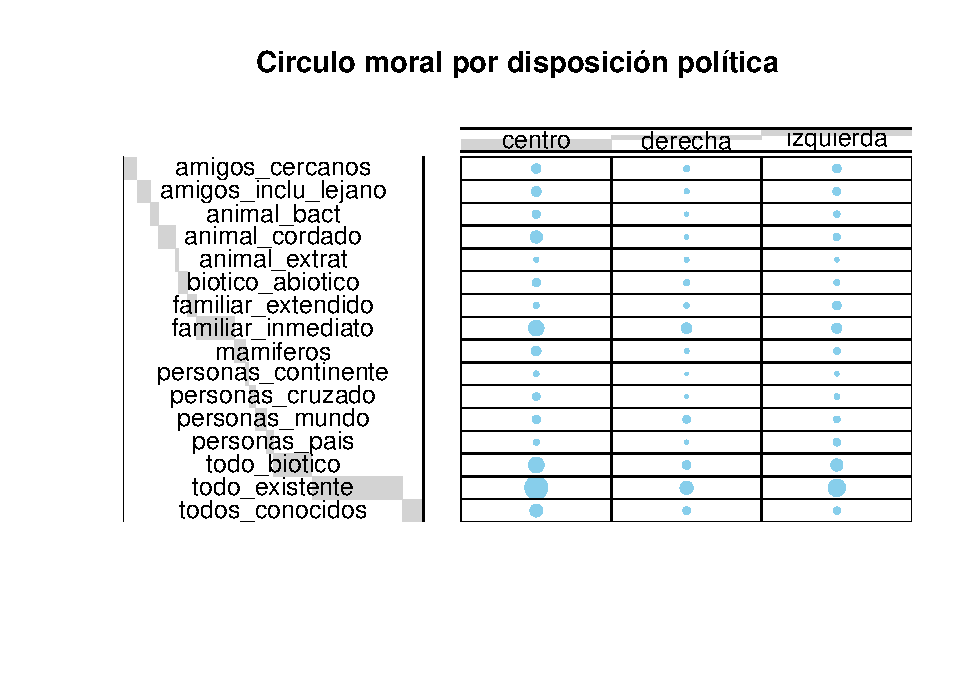
\includegraphics{3_analisis_correlacion_files/figure-latex/GRÁFICA esferas y barras-1.pdf}
\caption{Gráfica de perfiles}
\end{figure}

\hypertarget{prueba-de-independencia-ji2}{%
\subsubsection{\texorpdfstring{Prueba de independencia
\(ji^2\)}{Prueba de independencia ji\^{}2}}\label{prueba-de-independencia-ji2}}

Para evaluar la independencia entre las variables estudiadas se decide
realizar una prueba de \(ji^2\) a través de método de Pearson, con la
función \texttt{chisq.test}. Esta prueba corresponde a una prueba de
hipotesis entendida de la siguiente manera:

\[
H_o: las\ variables\  son\ independientes
\]

\[
H_1: las\ variables\  son\ dependientes
\]

\begin{longtable}[]{@{}cc@{}}
\caption{Prueba de independencia por \(Ji^2\)}\tabularnewline
\toprule
\begin{minipage}[b]{0.12\columnwidth}\centering
\(ji^2\)\strut
\end{minipage} & \begin{minipage}[b]{0.16\columnwidth}\centering
\(p-value\)\strut
\end{minipage}\tabularnewline
\midrule
\endfirsthead
\toprule
\begin{minipage}[b]{0.12\columnwidth}\centering
\(ji^2\)\strut
\end{minipage} & \begin{minipage}[b]{0.16\columnwidth}\centering
\(p-value\)\strut
\end{minipage}\tabularnewline
\midrule
\endhead
\begin{minipage}[t]{0.12\columnwidth}\centering
44.93\strut
\end{minipage} & \begin{minipage}[t]{0.16\columnwidth}\centering
0.03917\strut
\end{minipage}\tabularnewline
\bottomrule
\end{longtable}

El resultado de la \(ji^2\) puede verse en la tabla 5. El valor del
estadístico (44.93) fue obtenido con 30 grados de libertad con un
\(p - value = 0.03917\) lo que asumiendo un erro estandar de 5\% para la
prueba se puede concluir que no es posible rechazar la hipotesis nula
(\(H_0\)), de manera que las variables son dependientes.

\hypertarget{anuxe1lisis-de-corresponencia-y-gruxe1ficas}{%
\subsubsection{Análisis de corresponencia y
gráficas}\label{anuxe1lisis-de-corresponencia-y-gruxe1ficas}}

Se elabora un análisis de correspondencia a través de la función
\texttt{CA}del paquete \texttt{factoextra}. Se obtiene los valores
propios (o \emph{eigenvalues}) de las dimensiones mínimas obtenidas del
análisis de correspondencia (2). En otras palabras, con tan solo dos
dimensiones es posible explicar el 100 \% de la varianza de los datos
análizados, como se observa en la tabla 6. Del total de la varianza, la
dimensión 1 explicar el 54.3 \% de la varianza y la dimensión 2 el
45.7\% de esta.

La figura 2 corresponde al Scree plot de los \% de contribución de las
variables en general para cada una de las obtenidas, mostrando que los
perfiles entre variables explican en general casi de manera similar las
dimensiones 1 y 2.

\begin{longtable}[]{@{}cccc@{}}
\caption{Tabla de \emph{eigenvalues} y dimensiones}\tabularnewline
\toprule
\begin{minipage}[b]{0.14\columnwidth}\centering
~\strut
\end{minipage} & \begin{minipage}[b]{0.16\columnwidth}\centering
eigenvalue\strut
\end{minipage} & \begin{minipage}[b]{0.23\columnwidth}\centering
variance.percent\strut
\end{minipage} & \begin{minipage}[b]{0.36\columnwidth}\centering
cumulative.variance.percent\strut
\end{minipage}\tabularnewline
\midrule
\endfirsthead
\toprule
\begin{minipage}[b]{0.14\columnwidth}\centering
~\strut
\end{minipage} & \begin{minipage}[b]{0.16\columnwidth}\centering
eigenvalue\strut
\end{minipage} & \begin{minipage}[b]{0.23\columnwidth}\centering
variance.percent\strut
\end{minipage} & \begin{minipage}[b]{0.36\columnwidth}\centering
cumulative.variance.percent\strut
\end{minipage}\tabularnewline
\midrule
\endhead
\begin{minipage}[t]{0.14\columnwidth}\centering
\textbf{Dim.1}\strut
\end{minipage} & \begin{minipage}[t]{0.16\columnwidth}\centering
0.03551\strut
\end{minipage} & \begin{minipage}[t]{0.23\columnwidth}\centering
54.3\strut
\end{minipage} & \begin{minipage}[t]{0.36\columnwidth}\centering
54.3\strut
\end{minipage}\tabularnewline
\begin{minipage}[t]{0.14\columnwidth}\centering
\textbf{Dim.2}\strut
\end{minipage} & \begin{minipage}[t]{0.16\columnwidth}\centering
0.02989\strut
\end{minipage} & \begin{minipage}[t]{0.23\columnwidth}\centering
45.7\strut
\end{minipage} & \begin{minipage}[t]{0.36\columnwidth}\centering
100\strut
\end{minipage}\tabularnewline
\bottomrule
\end{longtable}

\begin{figure}
\centering
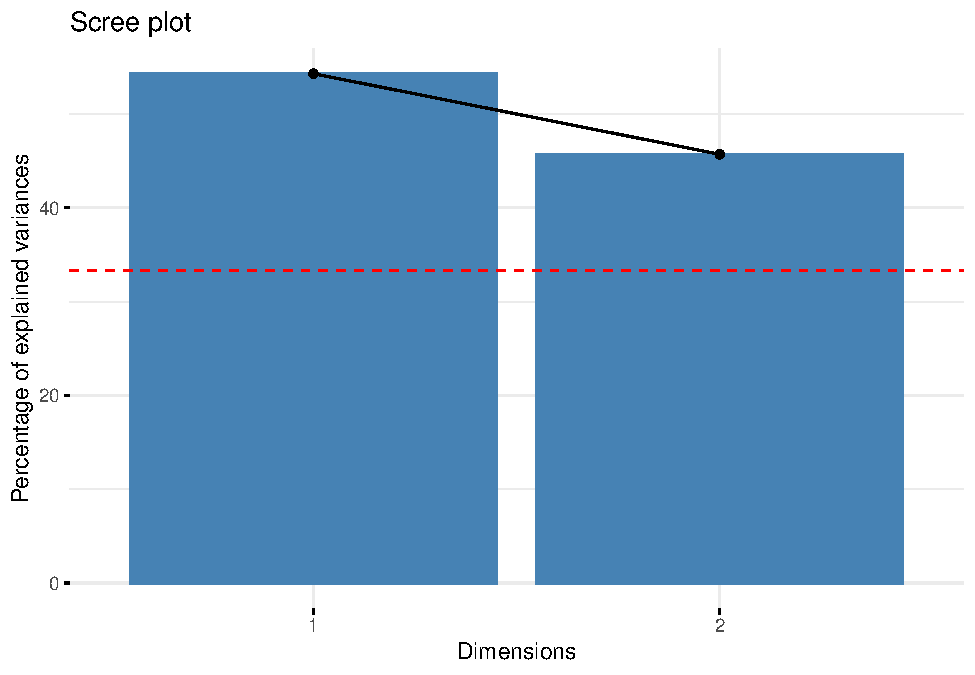
\includegraphics{3_analisis_correlacion_files/figure-latex/Gráfica de sedimentación-1.pdf}
\caption{gráfica de sedimentación}
\end{figure}

\hypertarget{biplots-y-contribuciones-de-las-variables.}{%
\subsubsection{Biplots y contribuciones de las
variables.}\label{biplots-y-contribuciones-de-las-variables.}}

Finalmente se realizaron dos tipos de Biplots, uno de estos simétrico
(figura 3) y un biplot asimétrico (figura 4.). Para darle mayor sentido
las gráficas se les asignó color en cuanto al peso de contribución para
la vector fila como a la variable columna.

\begin{figure}
\centering
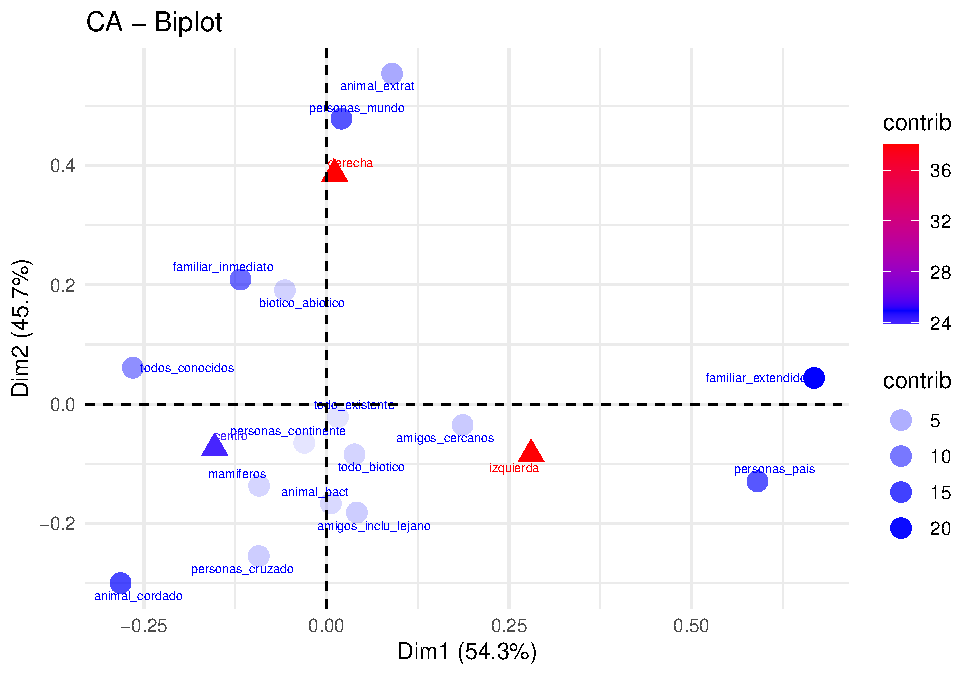
\includegraphics{3_analisis_correlacion_files/figure-latex/biplor de las categorias-1.pdf}
\caption{Biplot de las variables categóricas}
\end{figure}

En el caso del Biplot simétrico (figura 3.) se puede observar que las
vector columna fue representada con colores que van de rojo para la
máxima contribución de la variable a la dimensión y azul la menor
contribución. En el caso de la vector fila, se asigno azul oscuro para
la mayor contribución y azul más claro (o gris) para la menor
contribución. En el caso del biplot asimétrico se le asignó tanto a la
vector fila como al vector columna, color rojo a la máxima contribución
y azul a la mínima contribución.

\begin{figure}
\centering
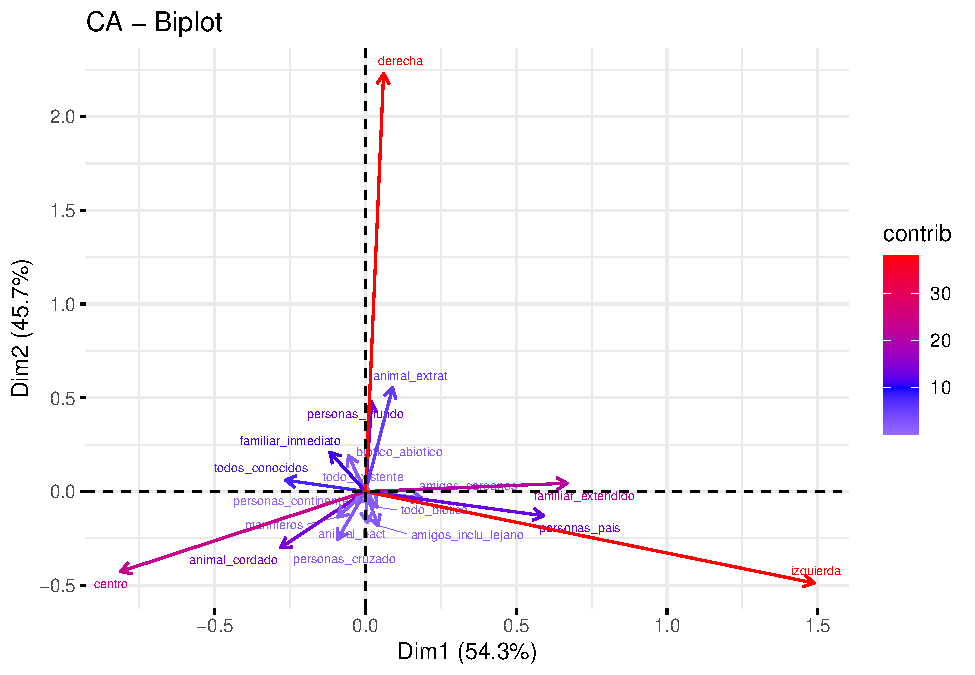
\includegraphics{3_analisis_correlacion_files/figure-latex/biplo asimétrico de las categorias-1.pdf}
\caption{Biplot de las variables categóricas}
\end{figure}

El Biplot simétrico deja ver algunos perfiles particulares entre las
variables. En primer lugar la categoría \texttt{derecha} se encuentra
muy cercana al eje y, lo que sugiere que esta vector es muy parecida al
perfil promedio o esperado para la observación. Sin embargo, como se
puede observar que es dentro de la variable columna la categoría que más
aporta a la segunda dimensión del plano factorial; lo mismo puede ser
dicho de la categoría \texttt{persona\_mundo} de la vector fila. En este
punto, se divisa un perfil de alta contribución de ambas categorías. Lo
que sugiere que el circulo moral de la personas que se autoperciben como
de derecha incluye una visión antropocentrica dónde es el ser humano el
centro de las categorías morales.

Por otra parte, la categoría \texttt{izquierda} dentro del vector
columna es el que más contribuye a la primera dimensión, al igual que
\texttt{persona\_pais}en el vector fila, aunque estos estén cercanos al
eje x, es decir al perfil promedio, es posible identificar un perfil
particular de relación entre estas dos categorías. Se podría sugerir de
esto, que las personas que se perciben como de izquierda pueden tener un
circulo moral de carcter más nacionalista.

En el caso de la categoría \texttt{centro} es la más cercana al 0 y se
encuentra en el lado negativo x, y, lo que sugiere que esta categoría es
la que menos contribuye a las dimensiones generadas, e incluso, las
categorías que aparecen en su rededor (también cercanas a 0) contribuyen
poco al análisis (esto se puede ver en la relación de color para cada
categoría).

Un análisis similar se puede obtener de la figura 4. En este biplot
asimétrico se puede observar la magnitud de los vectores contruidos para
cada categoría y su relación angular entre los vectores columna y los
vectores fila, además de sus contribuciones en las dimensiones. Como se
puede ver los vectores columna, \texttt{derecha} e \texttt{izquierda}
son los que más contribuyen al análisis de perfiles. En el caso de los
vectores fila, se observa que la mayor parte ellos tiene vectores cortos
desde el 0 lo que sugiere su baja contribución; sin embargo, cabe
destacar que \texttt{derecha} y \texttt{persona\_mundo} tienen un angulo
muy agudo lo que apunta a lo dicho anteriormente, la definición de un
perfil de relación entre las dos variables a través de estas categorías;
lo que es también perceptible en el caso de \texttt{izquierda} y
\texttt{persona\_pais}.

\end{document}
